A ship provisions a zone carrying several product references, so the decision is
the stock vector of Section~\ref{sec:decision} rather than a single number. Both
coverage criteria \eqref{eq:joint} and~\eqref{eq:agg} are evaluated exactly below,
and the dependence structure of~\eqref{eq:structure} acts on them in opposite
directions.

\subsection{Exact Distributions}
Let a ship carry $P$ populations with expected counts $\lambda_1,\dots,\lambda_P$
over the mission, $\Lambda=\sum_p\lambda_p$, and let the latent structure be
\eqref{eq:structure} with total variance $\sigma^2=\tau^2+\omega^2$ held fixed as
the allocation changes. Then
\begin{equation}
Y_p\mid u,w_p\sim\mathrm{Poisson}\!\left(\lambda_p
e^{u+w_p-\sigma^2/2}\right),
\label{eq:multi}
\end{equation}
with $u\sim\mathcal N(0,\tau^2)$ shared by the ship and
$w_p\sim\mathcal N(0,\omega^2)$ independent across references.

\begin{proposition}[Both criteria]
\label{prop:multi}
Given $u$ the references are conditionally independent. Writing
$g_{p,u}$ for the conditional mass function and $G_{p,u}$ for its distribution
function,
\begin{align}
g_{p,u}(m)&=\int \mathrm{Pois}\big(m;\lambda_p e^{u+w-\sigma^2/2}\big)\,
          \varphi_\omega(w)\,\mathrm dw,
\label{eq:convb}\\
\Pr\Big(\textstyle\sum_pY_p=n\Big)&=\int\Big[\ \ast_{p=1}^{P}\,g_{p,u}\Big](n)\,
          \varphi_\tau(u)\,\mathrm du,
\label{eq:conv}\\
\Pr\big(Y_p\le s_p\,\forall p\big)&=\int\prod_{p=1}^{P}G_{p,u}(s_p)\,
          \varphi_\tau(u)\,\mathrm du,
\label{eq:jointexact}
\end{align}
where $\ast$ denotes convolution over the counts. For $\omega=0$ the aggregate
\eqref{eq:conv} is a single mixed Poisson of mean $\Lambda$; for $\tau=0$ it is a
convolution of $P$ independent mixed Poissons.
\end{proposition}

Both are evaluated exactly, by discretising the two latent terms on a common
lattice so that every value of $u+w$ is a lattice point. Truncation contributes at
most $\mpTrunc$ of probability mass, and halving the lattice spacing leaves every
reported quantile unchanged.

\subsection{Joint Criterion: The Stock Vector}
Table~\ref{tab:stock} splits an expected \mpMean{} failures equally over $P$
references at a ship never seen, with total latent spread $\sigma=\mpSigma$, both
assumed values.

First, setting each reference at its own marginal 99\,\% quantile does not deliver
99\,\% joint cover: at $P=4$ that plan delivers \svNaiveShipFour\,\%, and at
$P=8$ it delivers \svNaiveShip\,\% under a ship-wide deviation and
\svNaiveInter\,\% under an interaction structure. Per-reference quantiles are
therefore not a solution to~\eqref{eq:joint}, and the shortfall grows with $P$.

Second, meeting~\eqref{eq:joint} at $P=8$ requires \svJointEight{} units of each
reference, \svJointTotEight{} in total, against \svMargTotEight{} for the
per-reference quantiles. Non-interchangeable references cannot pool risk, so the
total grows roughly linearly in $P$ at fixed total mean, unlike the aggregate
criterion.

Third, the direction of the dependence effect reverses between the two criteria.
Under~\eqref{eq:joint} a shared deviation makes the references move together,
which raises the probability that all are simultaneously covered: at $P=2$ the
ship-wide structure needs \svJointShipTwo{} units per reference against
\svJointInterTwo{} for the interaction structure, and the joint cover of the
per-reference plan is higher under the shared deviation (\svNaiveShip\,\% against
\svNaiveInter\,\% at $P=8$). Under~\eqref{eq:agg} the ordering is the opposite.

\subsection{Aggregate Criterion: Interchangeable References}
Where the references are interchangeable, the decision is the single number $S$
of~\eqref{eq:agg} and risk pools. Fig.~\ref{fig:multi} reports it. With one population the three
allocations agree exactly, at \mpShipOne{} units, as Section~\ref{sec:structure}
implies. As references are added the plans separate.
At $P=4$ the ship-wide structure requires \mpShipFour{} units against
\mpInterFour{} for the interaction structure, and at $P=8$ it requires
\mpShipEight{} against \mpInterEight{}. The mechanism is direct: a deviation
shared by every population does not average out under summation, so the total
retains the full latent spread however finely the estate is divided, whereas
independent deviations partially cancel and the total concentrates as $P$ grows.

The consequence of building the plan on the wrong allocation is asymmetric. The
lower panel of Fig.~\ref{fig:multi} evaluates a plan built assuming independent
interaction when the deviation is in fact ship-wide: at $P=8$ it delivers
\mpWrongCover\,\% where 99\,\% was intended. The opposite error is expensive
rather than unsafe: a plan assuming a ship-wide deviation delivers
\mpConsCover\,\% when the truth is independent, embarking \mpShipEight{} units
where \mpInterEight{} would have sufficed.

\begin{figure}[!t]
\centering
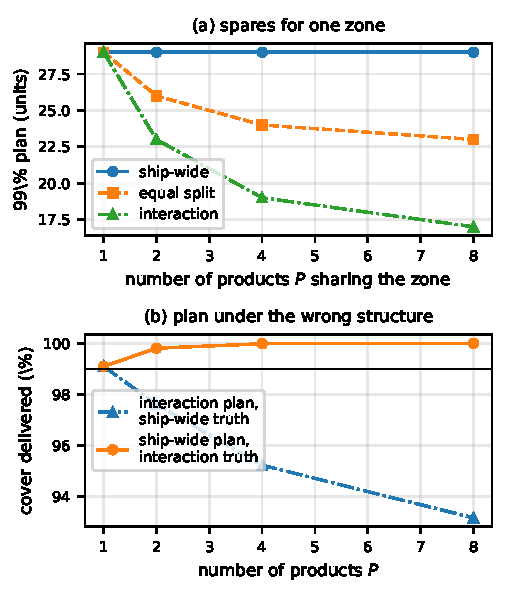
\includegraphics[width=\columnwidth]{figures/fig2_multiproduct.pdf}
\caption{Aggregate criterion~\eqref{eq:agg}, valid for interchangeable
references (\textsc{analytical}; the expected count \mpMean{} and the total
spread $\sigma=\mpSigma$ are assumed values). (top) The 99\,\% plan against the
number of references sharing the zone, under the two allocations of that spread
and an equal split. (bottom) Cover delivered when the plan is built under the
wrong allocation.}
\label{fig:multi}
\end{figure}

\begin{table}[!t]
\caption{Joint criterion~\eqref{eq:joint} against the aggregate
criterion~\eqref{eq:agg} at the 99\,\% level (\textsc{analytical}; expected
\mpMean{} failures over the zone and $\sigma=\mpSigma$ are assumed values).
$s_{\mathrm{marg}}$ is each reference's own marginal quantile and
$\gamma_{\mathrm{marg}}$ the joint cover it delivers; $s_{\mathrm{joint}}$ is the
smallest common per-reference stock meeting~\eqref{eq:joint}. The last two
columns compare total units under the two criteria: risk pools only when the
references are interchangeable}
\label{tab:stock}
\centering
\footnotesize
\setlength{\tabcolsep}{3.5pt}
\begin{tabular}{@{}clccccc@{}}
\toprule
& & \multicolumn{2}{c}{per-reference quantile} &
\multicolumn{2}{c}{joint~\eqref{eq:joint}} & agg.~\eqref{eq:agg} \\
\cmidrule(lr){3-4}\cmidrule(lr){5-6}\cmidrule(lr){7-7}
$P$ & structure & $s_{\mathrm{marg}}$ & $\gamma_{\mathrm{marg}}$ &
$s_{\mathrm{joint}}$ & total & total \\
\midrule
\tabinput{tables/tab_stock.tex}
\bottomrule
\end{tabular}
\end{table}

\subsection{Consequences}
Two conclusions for practice follow. The criterion must be fixed before the plan
is computed, since the two answers differ by a factor of order $P$ and respond to
the dependence structure with opposite signs: a fleet holding non-interchangeable
references uses~\eqref{eq:joint}, and the aggregate figure applies only to
interchangeable stock. Neither criterion should then be approached by adding
per-reference quantiles, since evaluating~\eqref{eq:conv}
and~\eqref{eq:jointexact}, or drawing from the fitted model, costs little.

The allocation between $\tau$ and $\omega$, however, is an empirical quantity that
no data in this paper determine, so a single data-holder $\sigma$ is not
sufficient to size a multi-reference plan under either criterion and none is
reported. While the ordering is unresolved, the defensible practice is to compute
the plan under both extremes and adopt the more conservative figure for the
criterion in force.
